\documentclass[letterpaper,10pt]{book}
% Change to 10 pt
\usepackage{pdfpages}
\usepackage{morewrites}			% to counteract the no write space problem
\setcounter{tocdepth}{6}

\usepackage[framemethod=TikZ]{mdframed}

\usepackage{fancyhdr}

\usepackage{paralist}
\usepackage{amsmath}
\usepackage{amsfonts}
\usepackage{amssymb}
\usepackage{graphicx}

\usepackage{datetime}
%\usepackage{ulem}

%\usepackage[nottoc]{toobibind}

\usepackage[inline]{enumitem}

% Outer margin at 2.50 is exacty correct to fit the ``corruption alert'' tables
\usepackage[inner=1.0in, outer=2.50in, top=2.54cm,bottom=2.54cm, marginparwidth=2.25in]{geometry}

\usepackage{marginnote}
\usepackage{longtable}
\usepackage{booktabs}
\usepackage{xcolor}

\usepackage{soul}

%%%%%%%%%%%%
\definecolor{ForestGreen}{rgb}{0.00,0.29,0.098}
%%%%%%%%%%%%

\usepackage{marginnote}

\usepackage{imakeidx} 
\usepackage[
	backref=true,
	style=numeric,
%	citestyle=numeric,
	backend=bibtex
	]{biblatex}
\usepackage[driverfallback=hypertex,colorlinks=True]{hyperref}
\usepackage{cleveref}

\makeindex[name=scripture,columnsep=20pt, columnseprule=True,columns=3, title=Scripture References]
\makeindex[name=speaker,columnsep=20pt, columnseprule=True,,columns=2, title=Sermon Creator]
\makeindex[name=series,columnsep=20pt, columnseprule=True,,columns=2, title=Sermon Series]
\makeindex[name=date,columnsep=20pt, columnseprule=True,columns=2, title=Sermon Date]
\makeindex[name=event,columnsep=20pt, columnseprule=True,columns=2, title=Event]
\makeindex[name=topic,columnsep=20pt, columnseprule=True,columns=2, title=Topic]
\makeindex[name=AWIP,columnsep=20pt, columnseprule=True,columns=3, title=All Words in Passage]
\makeindex[name=NWIV,columnsep=20pt, columnseprule=True,columns=3, title=Number of Words in Verse]
\makeindex[name=PNIP,columnsep=20pt, columnseprule=True,columns=3, title=Proper Names in Passage]
\makeindex[name=PEIP,columnsep=20pt, columnseprule=True,columns=2, title=Prophetic Events in Passage]
\makeindex[name=TWPAQ,columnsep=20pt, columnseprule=True,columns=1, title=13-Word Phrases and Quotes]
\makeindex[name=PFTTIS,columnsep=20pt, columnseprule=False,columns=3, title=Phrases found 13 times in scripture]
\makeindex[name=WFTTIS,columnsep=20pt, columnseprule=False,columns=3, title=Words found 13 times in scripture]
\makeindex[name=WFITV,columnsep=20pt, columnseprule=False,columns=3, title=Words found in exactly 13 verses]
\makeindex[name=EVENTS,columnsep=20pt, columnseprule=False,columns=2, title=Sermon Log by Place]
\makeindex[name=QUESTIONS,columnsep=20pt, columnseprule=False,columns=2, title=Bible Questions]
\makeindex[name=DOCTRINES,columnsep=20pt, columnseprule=False,columns=2, title=Doctrines]
\makeindex[name=SONGS,columnsep=20pt, columnseprule=False,columns=1, title=Songs]
\makeindex[name=LOCATION,columnsep=20pt, columnseprule=False,columns= 2, title=Location]
\makeindex[name=FACEBOOK,columnsep=20pt, columnseprule=False,columns=2, title=Facebook]
\makeindex[name=DEVOTIONAL,columnsep=20pt, columnseprule=False,columns=2, title=Devotional Items]
%%%%%%%%%%%%%%%%% EXTRA COLORS
\definecolor{champagne}{rgb}{0.97,0.91,0.81}
\definecolor{bone}{rgb}{0.89,0.85,0.79}
\pagestyle{fancy}
\fancyhf{}
\fancyhead[LE,RO]{\today}
\fancyhead[RE,LO]{Daily Bible Reading}
\fancyhead[CE,CO]{-page \thepage  - }

\fancyfoot[CO,CE]{\leftmark}
%\fancyfoot[LE,RO]{CSCE 692, HW1}

\title{DBR\\
Daily \\ Reads}
\author{Keith Anthony \\
\today }
%+/ffffff +   \pagenumbering{gobble}
\bibliography{Bibliographies/All20220122}

\setlength{\fboxsep}{1.0pt}

\usepackage[utf8]{inputenc}
\usepackage{tikz}

\begin{document}
%%%%%%%%%%%% Tile Page

\begin{titlepage}

\begin{flushright}
\rightskip=-2.5cm
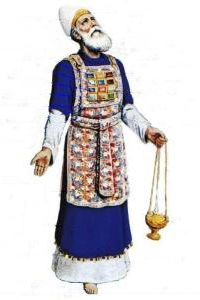
\includegraphics[width=50mm,scale=1.5]{Extras/Melchisedec.jpg}
\vspace{0.4in}  % Create a title for the document and write it in bold font
\LARGE{\textbf{\date}} % Again, do a line break
\linebreak 
% Create a subtitle \large{with Outlines, Statistics, Cross References, and Notes}
\vspace{0.5in}
\begin{flushleft}
\LARGE{Day \#68: Wednesday, 9 March 2022 PLAIN \\}\vspace{0.25in}
\LARGE{Joshua 10-12 Psalm 68 Proverb 9}
\end{flushleft}
\vspace{0.6in}
\bigskip

\normalsize{Xenia, Oh.\\}
\normalsize{created: \today}
\vspace{1.3in}

\end{flushright}
\end{titlepage}

\newpage 
\tableofcontents\hypertarget{TOC}{}
\listoffigures
\listoftables

\hyphenation{A-bim-e-lech bre-thren E-phra-im  Gib-e-o-nites Jer-u-sa-lem through-out Phil-i-stines The-o-phil-us Am-a-le-kites ven-geance Mesh-el-e-mi-ah onan-ism Phar-a-oh thoughts grev-ous-ness Hach-a-liah adul-ter-er Shad-rach}

%%%%%%%%%%%%%%%%% EXTRA COLORS
%%%%%%%%%%%%%%%%% EXTRA COLORS
%%%%%%%%%%%%%%%%% EXTRA COLORS
\definecolor{champagne}{rgb}{0.97,0.91,0.81}
\definecolor{bone}{rgb}{0.89,0.85,0.79}

\definecolor{ForestGreen}{rgb}{0.00,0.29,0.098}
\definecolor{GIVING}{cmyk}{1,0.0,0.72,.1}

\definecolor{MLPE}{cmyk}{1,1,0,.45}
\definecolor{SOCCER}{cmyk}{.77, 0, .42, .49}
\definecolor{PAYBILL}{cmyk}{0,0.83,0.76,0.07}
\definecolor{SERMON}{cmyk}{.14,.9,0,.30} % aka seance \href{http://www.flatuicolorpicker.com/purple-cmyk-color-model/}{seance}
\definecolor{BIBLE}{cmyk}{0,.17,.74,.17}
\definecolor{WORKBLUE}{cmyk}{1, .5, 0, .6}
\definecolor{myOrange}{cmyk}{0, .4, .98, .03}
\definecolor{myTan}{cmyk}{0.0,.07,.17,.10}
\definecolor{myRed}{cmyk}{0,1,1,0}
\definecolor{myWhite}{cmyk}{0,0,0,0}
\definecolor{BLUESoD}{cmyk}{.97,.84,0,.04}
\definecolor{WHITE}{cmyk}{0,0,0,0}
\definecolor{OLDGOLD}{cmyk}{0.05,0.3,1.00,0}
\definecolor{CASTLETON}{cmyk}{1,0,0.31,0.66}
\definecolor{cadmiumgreen}{rgb}{0.0, 0.42, 0.24}
\definecolor{jungle}{rgb}{0.203,0.4882,0.1718}
\definecolor{MYGOLD}{rgb}{1,.84,0}

\definecolor{MYLIGHTGRAY}{rgb}{.85,.85,.85}

\definecolor{codegreen}{rgb}{0,0.6,0}
\definecolor{codegray}{rgb}{0.5,0.5,0.5}
\definecolor{codepurple}{rgb}{0.58,0,0.82}
\definecolor{backcolour}{rgb}{0.95,0.95,0.92}


\mdfdefinestyle{MyFrame}{%
    linecolor=blue,
    outerlinewidth=2pt,
    roundcorner=5pt,
    innertopmargin=\baselineskip,
    innerbottommargin=\baselineskip,
    innerrightmargin=10pt,
    innerleftmargin=10pt,
    backgroundcolor=gray!25!white}


\mdfdefinestyle{MyFrame2}{%
    linecolor=black,
    outerlinewidth=2pt,
    roundcorner=5pt,
    innertopmargin=\baselineskip,
    innerbottommargin=\baselineskip,
    innerrightmargin=10pt,
    innerleftmargin=10pt,
    backgroundcolor=yellow!25!white}


%%%%%
%% for PFTTIS list
%%%%%

%%% And Joseph said unto
\index[PFTTIS]{And Joseph said unto!Genesis!Gen 40:008}
\index[PFTTIS]{And Joseph said unto!Genesis!Gen 40:012}
\index[PFTTIS]{And Joseph said unto!Genesis!Gen 41:025}
\index[PFTTIS]{And Joseph said unto!Genesis!Gen 42:014}
\index[PFTTIS]{And Joseph said unto!Genesis!Gen 42:018}
\index[PFTTIS]{And Joseph said unto!Genesis!Gen 44:015}
\index[PFTTIS]{And Joseph said unto!Genesis!Gen 45:003}
\index[PFTTIS]{And Joseph said unto!Genesis!Gen 45:004}
\index[PFTTIS]{And Joseph said unto!Genesis!Gen 46:031}
\index[PFTTIS]{And Joseph said unto!Genesis!Gen 48:009}
\index[PFTTIS]{And Joseph said unto!Genesis!Gen 48:018}
\index[PFTTIS]{And Joseph said unto!Genesis!Gen 50:019}
\index[PFTTIS]{And Joseph said unto!Genesis!Gen 50:024}


%%% a shadow
\index[PFTTIS]{a shadow!1Chronicles!1Chr 029:15}
\index[PFTTIS]{a shadow!Job!Job 008:09}
\index[PFTTIS]{a shadow!Job!Job 014:02}
\index[PFTTIS]{a shadow!Job!Job 017:07}
\index[PFTTIS]{a shadow!Psalm!Psa 102:011}
\index[PFTTIS]{a shadow!Psalm!Psa 144:004}
\index[PFTTIS]{a shadow!Ecclesiastes!Eccl 006:012}
\index[PFTTIS]{a shadow!Ecclesiastes!Eccl 008:013}
\index[PFTTIS]{a shadow!Isaiah!Isa 04:006}
\index[PFTTIS]{a shadow!Isaiah!Isa 25:004}
\index[PFTTIS]{a shadow!Jonah!Jnh 04:06}
\index[PFTTIS]{a shadow!Colossians!Col 02:017}
\index[PFTTIS]{a shadow!Hebews!Heb 10:001}

%%% blessed is the man
\index[PFTTIS]{blessed is the man!Psalm!Psa 001:001}
\index[PFTTIS]{blessed is the man!Psalm!Psa 032:002}
\index[PFTTIS]{blessed is the man!Psalm!Psa 034:008}
\index[PFTTIS]{blessed is the man!Psalm!Psa 065:004}
\index[PFTTIS]{blessed is the man!Psalm!Psa 084:005}
\index[PFTTIS]{blessed is the man!Psalm!Psa 084:012}
\index[PFTTIS]{blessed is the man!Psalm!Psa 094:012}
\index[PFTTIS]{blessed is the man!Psalm!Psa 112:001}
\index[PFTTIS]{blessed is the man!Proverbs!Pro 008:034}
\index[PFTTIS]{blessed is the man!Isaiah!Isa 056:002}
\index[PFTTIS]{blessed is the man!Jeremiah!Jer 017:007}
\index[PFTTIS]{blessed is the man!Romans!Rom 004:008}
\index[PFTTIS]{blessed is the man!James!Jam 001:012}


%%% carry them
\index[PFTTIS]{carry them!Leviticus!Lev 14:045}
\index[PFTTIS]{carry them!Numbers!Num 11:012}
\index[PFTTIS]{carry them!Joshua!Jsh 04:003}
\index[PFTTIS]{carry them!1Samuel!1Sam 20:040}
\index[PFTTIS]{carry them!1Kings!1Kng 08:046}
\index[PFTTIS]{carry them!2Chronicles!2Chr 06:036}
\index[PFTTIS]{carry them!Ezra!Ezra 05:015}
\index[PFTTIS]{carry them!Isaiah!Isa 40:011}
\index[PFTTIS]{carry them!Isaiah!Isa 41:016}
\index[PFTTIS]{carry them!Isaiah!Isa 57:013}
\index[PFTTIS]{carry them!Jeremiah!Jer 20:004}
\index[PFTTIS]{carry them!Jeremiah!Jer 20:005}
\index[PFTTIS]{carry them!Jeremiah!Jer 43:012}


\index[PFTTIS]{good tidings!2Samuel!2Sam 18:027}
\index[PFTTIS]{good tidings!1Kings!1Ki 01:042}
\index[PFTTIS]{good tidings!2Kings!2Ki 07:009 (2x)}
\index[PFTTIS]{good tidings!Isaiah!Isa 40:009 (2x)}
\index[PFTTIS]{good tidings!Isaiah!Isa 41:007}
\index[PFTTIS]{good tidings!Isaiah!Isa 52:007}
\index[PFTTIS]{good tidings!Isaiah!Isa 61:001}
\index[PFTTIS]{good tidings!Nahum!Nah 01:005}
\index[PFTTIS]{good tidings!Luke!Lk 02:010}
\index[PFTTIS]{good tidings!1Thessalonians!1Thess 03:006}


%%% dead body
\index[PFTTIS]{dead body!Leviticus!Lev 21:011}
\index[PFTTIS]{dead body!Numbers!Num 06:006}
\index[PFTTIS]{dead body!Numbers!Num 09:006}
\index[PFTTIS]{dead body!Numbers!Num 09:007}
\index[PFTTIS]{dead body!Numbers!Num 09:010}
\index[PFTTIS]{dead body!Numbers!Num 09:011}
\index[PFTTIS]{dead body!Numbers!Num 09:013}
\index[PFTTIS]{dead body!Numbers!Num 09:016}
\index[PFTTIS]{dead body!2Kings!2Ki 08:005}
\index[PFTTIS]{dead body!Isaiah!Isa 26:019}
\index[PFTTIS]{dead body!Jeremiah!Jer 26:023}
\index[PFTTIS]{dead body!Jeremiah!Jer 36:030}
\index[PFTTIS]{dead body!Haggai!Hag 02:013}

%%% great sea
\index[PFTTIS]{great sea!Numbers!Num 34:006}
\index[PFTTIS]{great sea!Numbers!Num 34:007}
\index[PFTTIS]{great sea!Joshua!Jos 01:004}
\index[PFTTIS]{great sea!Joshua!Jos 09:001}
\index[PFTTIS]{great sea!Joshua!Jos 15:012}
\index[PFTTIS]{great sea!Joshua!Jos 15:047}
\index[PFTTIS]{great sea!Joshua!Jos 23:004}
\index[PFTTIS]{great sea!Ezekiel!Eze 47:010}
\index[PFTTIS]{great sea!Ezekiel!Eze 47:015}
\index[PFTTIS]{great sea!Ezekiel!Eze 47:019}
\index[PFTTIS]{great sea!Ezekiel!Eze 47:020}
\index[PFTTIS]{great sea!Ezekiel!Eze 48:028}
\index[PFTTIS]{great sea!Daniel!Dan 07:002}


%%% have forsaken me
\index[PFTTIS]{have forsaken me!Judges!Jdg 10:013}
\index[PFTTIS]{have forsaken me!1Samuel!1Sam 08:008}
\index[PFTTIS]{have forsaken me!1Kings!1Ki 11:033}
\index[PFTTIS]{have forsaken me!2Kings!2Ki 22:017}
\index[PFTTIS]{have forsaken me!2Chronicles!2Chr 12:005}
\index[PFTTIS]{have forsaken me!2Chronicles!2Chr 34:025}
\index[PFTTIS]{have forsaken me!Jeremiah!Jer 01:016}
\index[PFTTIS]{have forsaken me!Jeremiah!Jer 02:013}
\index[PFTTIS]{have forsaken me!Jeremiah!Jer 05:007}
\index[PFTTIS]{have forsaken me!Jeremiah!Jer 05:019}
\index[PFTTIS]{have forsaken me!Jeremiah!Jer 16:011 (2x)}
\index[PFTTIS]{have forsaken me!Jeremiah!Jer 19:004}

%%% no king
\index[PFTTIS]{no king!Judges!Jdg 17:06}
\index[PFTTIS]{no king!Judges!Jdg 18:01}
\index[PFTTIS]{no king!Judges!Jdg 19:01}
\index[PFTTIS]{no king!Judges!Jdg 21:25}
\index[PFTTIS]{no king!1Kings!1Ki 22:47}
\index[PFTTIS]{no king!2Kings!2Ki 23:25}
\index[PFTTIS]{no king!Nehemiah!Neh 13:26}
\index[PFTTIS]{no king!Psalms!Psa 033:016}
\index[PFTTIS]{no king!Proverbs!Pro 30:27}
\index[PFTTIS]{no king!Daniel!Dan 02:10}
\index[PFTTIS]{no king!Hosea!Hos 10:03}
\index[PFTTIS]{no king!Micah!Mic 04:09}
\index[PFTTIS]{no king!John!Jhn 19:15}


%%% rebellious house
\index[PFTTIS]{rebellious house!Exodus!Exo 02:005}
\index[PFTTIS]{rebellious house!Exodus!Exo 02:006}
\index[PFTTIS]{rebellious house!Exodus!Exo 02:008}
\index[PFTTIS]{rebellious house!Exodus!Exo 03:009}
\index[PFTTIS]{rebellious house!Exodus!Exo 03:026}
\index[PFTTIS]{rebellious house!Exodus!Exo 03:027}
\index[PFTTIS]{rebellious house!Exodus!Exo 12:002 (2x)}
\index[PFTTIS]{rebellious house!Exodus!Exo 12:003}
\index[PFTTIS]{rebellious house!Exodus!Exo 12:009}
\index[PFTTIS]{rebellious house!Exodus!Exo 12:025}
\index[PFTTIS]{rebellious house!Exodus!Exo 17:012}
\index[PFTTIS]{rebellious house!Exodus!Exo 24:003}

%%% seek him
\index[PFTTIS]{seek him!Deuteronomy!Deu 04:029}\index[PFTTIS]{seek him!1Samuel!1Sam 23:025}
\index[PFTTIS]{seek him!1Chronicles!1Chr 28:009}
\index[PFTTIS]{seek him!2Chronicles!1Chr 15:002}
\index[PFTTIS]{seek him!Ezra!Ezr 08:022}
\index[PFTTIS]{seek him!Psalms!Psa 022:026}
\index[PFTTIS]{seek him!Psalms!Psa 024:006}
\index[PFTTIS]{seek him!Psalms!Psa 119:002}
\index[PFTTIS]{seek him!SoS!SoS 03:002}
\index[PFTTIS]{seek him!SoS!SoS 06:001}
\index[PFTTIS]{seek him!Hosea!Hos 07:010}
\index[PFTTIS]{seek him!Amos!Amo 05:008}
\index[PFTTIS]{seek him!Hebrews!Heb 11:0063}


%%% seek ye
\index[PFTTIS]{seek ye!Isaiah!Isa 34:016}
\index[PFTTIS]{seek ye!Isaiah!Isa 45:019}
\index[PFTTIS]{seek ye!Isaiah!Isa 55:006}
\index[PFTTIS]{seek ye!Amos!Amos 5:004}
\index[PFTTIS]{seek ye!John!John 1:38}
\index[PFTTIS]{seek ye!John!John 18:4}
\index[PFTTIS]{seek ye!John!John 18:7}
\index[PFTTIS]{seek ye!Matthew!Matt 6:33}
\index[PFTTIS]{seek ye!Numbers!Num 16:10}
\index[PFTTIS]{seek ye!Luke!Luke 12:31}
\index[PFTTIS]{seek ye!Luke!Luke 24:5}
\index[PFTTIS]{seek ye!Psalm!Psa 27:8}
\index[PFTTIS]{seek ye!Zephaniah!Zeph 2:3}

%%% the uncircumcised
\index[PFTTIS]{the uncircumcised!Genesis!Gen 17:014}
\index[PFTTIS]{the uncircumcised!Judges!Jdg 14:003}
\index[PFTTIS]{the uncircumcised!Judges!Jdg 15:018}
\index[PFTTIS]{the uncircumcised!2Samuel!2Sam 01:020}
\index[PFTTIS]{the uncircumcised!Isaiah!Isa 02:001}
\index[PFTTIS]{the uncircumcised!Jeremiah!Jer 09:025}
\index[PFTTIS]{the uncircumcised!Ezekiel!Eze 28:010}
\index[PFTTIS]{the uncircumcised!Ezekiel!Eze 31:018}
\index[PFTTIS]{the uncircumcised!Ezekiel!Eze 32:019}
\index[PFTTIS]{the uncircumcised!Ezekiel!Eze 32:027}
\index[PFTTIS]{the uncircumcised!Ezekiel!Eze 32:028}
\index[PFTTIS]{the uncircumcised!Ezekiel!Eze 32:029}
\index[PFTTIS]{the uncircumcised!Ezekiel!Eze 32:032}

%%% worship him
\index[PFTTIS]{worship him!Psalms!Psa 97:007}
\index[PFTTIS]{worship him!Zephaniah!Zeph 02:011}
\index[PFTTIS]{worship him!Matthew!Matt 02:002}
\index[PFTTIS]{worship him!Matthew!Matt 02:008}
\index[PFTTIS]{worship him!John!John 04:023}
\index[PFTTIS]{worship him!John!John 04:024 (2x)} 
\index[PFTTIS]{worship him!Acts!Acts 17:023}
\index[PFTTIS]{worship him!Hebrews!Heb 01:006}
\index[PFTTIS]{worship him!Revelation!Rev 04:010}
\index[PFTTIS]{worship him!Revelation!Rev 13:008}
\index[PFTTIS]{worship him!Revelation!Rev 14:007}
\index[PFTTIS]{worship him!Revelation!Rev 19:010}


%%%%%
%% for PFTTIS list
%%%%%

%%% afflictions
\index[WFTTIS]{afflictions!Psalms!Psa 34:019}
\index[WFTTIS]{afflictions!Psalms!Psa 132:001}
\index[WFTTIS]{afflictions!Acts!Acts 07:010}
\index[WFTTIS]{afflictions!Acts!Acts 20:023}
\index[WFTTIS]{afflictions!2Corinthians!2Cor 06:004}
\index[WFTTIS]{afflictions!Colossians!Col 01:024}
\index[WFTTIS]{afflictions!1Thessalonians!1Thess 03:003}
\index[WFTTIS]{afflictions!2Timothy!2Tim 01:008}
\index[WFTTIS]{afflictions!2Timothy!2Tim 03:011}
\index[WFTTIS]{afflictions!2Timothy!2Tim 04:005}
\index[WFTTIS]{afflictions!Hebrews!Heb 10:032}
\index[WFTTIS]{afflictions!Hebrews!Heb 10:033}
\index[WFTTIS]{afflictions!1Peter!1Pet 05:009}

%%% acsend
\index[WFTTIS]{acsend!Joshua!Jos 06:05}
\index[WFTTIS]{acsend!Psalm!Psa 024:003}
\index[WFTTIS]{acsend!Psalm!Psa 135:007}
\index[WFTTIS]{acsend!Psalm!Psa 139:008}
\index[WFTTIS]{acsend!Isaiah!Isa 14:013}
\index[WFTTIS]{acsend!Isaiah!Isa 14:014}
\index[WFTTIS]{acsend!Jeremiah!Jer 10:013}
\index[WFTTIS]{acsend!Jeremiah!Jer 51:016}
\index[WFTTIS]{acsend!Ezekiel!Eze 38:009}
\index[WFTTIS]{acsend!John!John 06:062}
\index[WFTTIS]{acsend!John!John 20:017}
\index[WFTTIS]{acsend!Romans!Rom 10:006}
\index[WFTTIS]{acsend!Revelation!Rev 17:008}

%%% Assyrian
\index[WFTTIS]{Assyrian!Isaiah!Isa 10:005}
\index[WFTTIS]{Assyrian!Isaiah!Isa 10:024}
\index[WFTTIS]{Assyrian!Isaiah!Isa 14:025}
\index[WFTTIS]{Assyrian!Isaiah!Isa 19:023}
\index[WFTTIS]{Assyrian!Isaiah!Isa 23:013}
\index[WFTTIS]{Assyrian!Isaiah!Isa 30:031}
\index[WFTTIS]{Assyrian!Isaiah!Isa 31:008}
\index[WFTTIS]{Assyrian!Isaiah!Isa 52:004}
\index[WFTTIS]{Assyrian!Ezekiel!Eze 31:003}
\index[WFTTIS]{Assyrian!Hosea!Hos 05:013}
\index[WFTTIS]{Assyrian!Hosea!Hos 11:005}
\index[WFTTIS]{Assyrian!Micah!Hos 05:005}
\index[WFTTIS]{Assyrian!Micah!Hos 05:006}

%%% blot
\index[WFTTIS]{blot!Exodus!Exo 32:032}
\index[WFTTIS]{blot!Exodus!Exo 32:033}
\index[WFTTIS]{blot!Numbers!Num 05:026}
\index[WFTTIS]{blot!Deuteronomy!Deut 09:014}
\index[WFTTIS]{blot!Deuteronomy!Deut 25:019}
\index[WFTTIS]{blot!Deuteronomy!Deut 29:020}
\index[WFTTIS]{blot!2Kings!2Ki 14:027}
\index[WFTTIS]{blot!Job!Job 31:007}
\index[WFTTIS]{blot!Psalms!Psa 51:001}
\index[WFTTIS]{blot!Psalms!Psa 51:009}
\index[WFTTIS]{blot!Proverbs!Pro 09:007}
\index[WFTTIS]{blot!Jeremiah!Jer 18:023}
\index[WFTTIS]{blot!Revelation!Rev 03:005}


%%% chain
\index[WFTTIS]{chain!Genesis!Gen 41:042}
\index[WFTTIS]{chain!1Kings!1Ki 07:017}
\index[WFTTIS]{chain!Psalms!Psa 73:006}
\index[WFTTIS]{chain!SoS!Sos 04:009}
\index[WFTTIS]{chain!Lamentations!Lam 03:007}
\index[WFTTIS]{chain!Ezekiel!Eze 07:023}
\index[WFTTIS]{chain!Ezekiel!Eze 16:011}
\index[WFTTIS]{chain!Daniel!Dan 05:007}
\index[WFTTIS]{chain!Daniel!Dan 05:016}
\index[WFTTIS]{chain!Daniel!Dan 05:029}
\index[WFTTIS]{chain!Acts!Acts 28:020}
\index[WFTTIS]{chain!2Timothy!2Tim 01:016}
\index[WFTTIS]{chain!Revelation!Rev 20:001}


%%% controversy
\index[WFTTIS]{controversy!Deuteronomy!Deu 17:008}
\index[WFTTIS]{controversy!Deuteronomy!Deu 19:017}
\index[WFTTIS]{controversy!Deuteronomy!Deu 21:005}
\index[WFTTIS]{controversy!Deuteronomy!Deu 25:001}
\index[WFTTIS]{controversy!2Samuel!2Sam 15:002}
\index[WFTTIS]{controversy!Isaiah!Isa 34:008}
\index[WFTTIS]{controversy!Jeremiah!Jer 25:031}
\index[WFTTIS]{controversy!Ezekiel!Eze 44:024}
\index[WFTTIS]{controversy!Hosea!Hos 04:001}
\index[WFTTIS]{controversy!Hosea!Hos 12:002}
\index[WFTTIS]{controversy!Micah!Mic 06:002 (2x)}
\index[WFTTIS]{controversy!1Timothy!1Tim 03:016}


%%% Dagon/Dagon's
\index[WFTTIS]{Dagon!Judges!Jdg 16:023}
\index[WFTTIS]{Dagon!1Samuel!1Sam 05:002 (2x)}
\index[WFTTIS]{Dagon!1Samuel!1Sam 05:003 (2x)}
\index[WFTTIS]{Dagon!1Samuel!1Sam 05:004 (3x)}
\index[WFTTIS]{Dagon!1Samuel!1Sam 05:005 (3x)}
\index[WFTTIS]{Dagon!1Samuel!1Sam 05:007}
\index[WFTTIS]{Dagon!1Chronicles!1Chr 10:010}

%%% disobedient
\index[WFTTIS]{disobedient!1Kings!1Ki 13:026}
\index[WFTTIS]{disobedient!Nehemiah!Neh 09:026}
\index[WFTTIS]{disobedient!Luke!Luke 01:017}
\index[WFTTIS]{disobedient!Acts!Acts 26:019}
\index[WFTTIS]{disobedient!Romans!Rom 01:030}
\index[WFTTIS]{disobedient!Romans!Rom 10:021}
\index[WFTTIS]{disobedient!1Timothy!1Tim 01:009}
\index[WFTTIS]{disobedient!2Timothy!2Tim 03:002}
\index[WFTTIS]{disobedient!Titus!Titus 01:016}
\index[WFTTIS]{disobedient!Titus!Titus 03:003}
\index[WFTTIS]{disobedient!1Peter!1Pet 02:007}
\index[WFTTIS]{disobedient!1Peter!1Pet 02:008}
\index[WFTTIS]{disobedient!1Peter!1Pet 03:020}


%%% doubt
\index[WFTTIS]{doubt!Genesis!Gen 37:033}
\index[WFTTIS]{doubt!Deuteronomy!Deu 28:066}
\index[WFTTIS]{doubt!Job!Job 12:002}
\index[WFTTIS]{doubt!Matthew!Matt 14:031}
\index[WFTTIS]{doubt!Matthew!Matt 21:021}
\index[WFTTIS]{doubt!Mark!Mk 11:023}
\index[WFTTIS]{doubt!Luke!Lk 11:020}
\index[WFTTIS]{doubt!John!Jhn 10:024}
\index[WFTTIS]{doubt!Acts!Acts 02:012}
\index[WFTTIS]{doubt!Acts!Acts 28:004}
\index[WFTTIS]{doubt!1Corinthians!1Cor 09:010}
\index[WFTTIS]{doubt!Galatians!Gal 04:020}
\index[WFTTIS]{doubt!1John!1Jhn 02:019}


%%% dungeon
\index[WFTTIS]{dungeon!Genesis!Gen 40:015}
\index[WFTTIS]{dungeon!Genesis!Gen 41:014}
\index[WFTTIS]{dungeon!Exodus!Exo 12:029}
\index[WFTTIS]{dungeon!Jeremiah!Jer 37:016}
\index[WFTTIS]{dungeon!Jeremiah!Jer 38:006 (2x)}
\index[WFTTIS]{dungeon!Jeremiah!Jer 38:007}
\index[WFTTIS]{dungeon!Jeremiah!Jer 38:009}
\index[WFTTIS]{dungeon!Jeremiah!Jer 38:010}
\index[WFTTIS]{dungeon!Jeremiah!Jer 38:011}
\index[WFTTIS]{dungeon!Jeremiah!Jer 38:013}
\index[WFTTIS]{dungeon!Lamentations!Lam 03:053}
\index[WFTTIS]{dungeon!Lamentations!Lam 03:055}


%%% error
\index[WFTTIS]{error!2Samuel!2Sam 06:007}
\index[WFTTIS]{error!Job!Job 19:004}
\index[WFTTIS]{error!Ecclesiastes!Ecc 05:006}
\index[WFTTIS]{error!Ecclesiastes!Ecc 10:005}
\index[WFTTIS]{error!Isaiah!Isa 32:006}
\index[WFTTIS]{error!Daniel!Dan 06:004}
\index[WFTTIS]{error!Matthew!Matt 27:064}
\index[WFTTIS]{error!Romans!Rom 01:027}
\index[WFTTIS]{error!James!Jam 05:020}
\index[WFTTIS]{error!2Peter!2Pet 02:018}
\index[WFTTIS]{error!2Peter!2Pet 03:017}
\index[WFTTIS]{error!1John!1Jn 04:006}
\index[WFTTIS]{error!Jude!Jude 01:011}

%%% fourish
\index[WFTTIS]{fourish!Psalms!Psa 072:007}
\index[WFTTIS]{fourish!Psalms!Psa 072:016}
\index[WFTTIS]{fourish!Psalms!Psa 092:007}
\index[WFTTIS]{fourish!Psalms!Psa 092:012}
\index[WFTTIS]{fourish!Psalms!Psa 092:013}
\index[WFTTIS]{fourish!Psalms!Psa 132:018}
\index[WFTTIS]{fourish!Proverbs!Pro 11:28}
\index[WFTTIS]{fourish!Proverbs!Pro 14:11}
\index[WFTTIS]{fourish!Ecclesiastes!Ecc 12:05}
\index[WFTTIS]{fourish!SongOfSolomon!SOS 07:12}
\index[WFTTIS]{fourish!Isaiah!Isa 17:11}
\index[WFTTIS]{fourish!Isaiah!Isa 66:14}
\index[WFTTIS]{fourish!Ezekiel!Eze 17:24}




%%% giants
\index[WFTTIS]{giants!Genesis!Gen 06:004}
\index[WFTTIS]{giants!Numbers!Num 13:033}
\index[WFTTIS]{giants!Deuteronomy!Deut 02:011}
\index[WFTTIS]{giants!Deuteronomy!Deut 02:021}
\index[WFTTIS]{giants!Deuteronomy!Deut 03:011}
\index[WFTTIS]{giants!Deuteronomy!Deut 03:013}
\index[WFTTIS]{giants!Joshua!Josh 12:004}
\index[WFTTIS]{giants!Joshua!Josh 13:012}
\index[WFTTIS]{giants!Joshua!Josh 15:008}
\index[WFTTIS]{giants!Joshua!Josh 17:015}
\index[WFTTIS]{giants!Joshua!Josh 16:016}

%%% good man
\index[WFTTIS]{good man!2 Samuel!2Sa 18:27}
%(1) Psalms 37:23 [5]
%(1) Psalms 112:5 [2]
%(1) Proverbs 12:2 [2]
%(1) Proverbs 13:22 [2]
%(1) Proverbs 14:14 [14]
%(1) Micah 7:2 [2]
%(1) Matthew 12:35 [2]
%(1) Luke 6:45 [2]
%(1) Luke 23:50 [15]
%(1) John 7:12 [17]
%(1) Acts 11:24 [5]
%(1) Romans 5:7 [14]

%%% Hinnom
\index[WFTTIS]{Hinnom!Joshua!Jsh 15:008}
\index[WFTTIS]{Hinnom!Joshua!Jsh 18:016}
\index[WFTTIS]{Hinnom!2Kings!2Ki 23:010}
\index[WFTTIS]{Hinnom!2Chronicles!2Chr 28:003}
\index[WFTTIS]{Hinnom!2Chronicles!2Chr 33:006}
\index[WFTTIS]{Hinnom!Nehemiah!Neh 11:030}
\index[WFTTIS]{Hinnom!Jeremiah!Jer 07:031}
\index[WFTTIS]{Hinnom!Jeremiah!Jer 07:032}
\index[WFTTIS]{Hinnom!Jeremiah!Jer 19:002}
\index[WFTTIS]{Hinnom!Jeremiah!Jer 19:006}
\index[WFTTIS]{Hinnom!Jeremiah!Jer 32:035}

%%% inclined
\index[WFTTIS]{inclined!Judges!Jdg 09:003}
\index[WFTTIS]{inclined!Psalms!Psa 040:001}
\index[WFTTIS]{inclined!Psalms!Psa 116:002}
\index[WFTTIS]{inclined!Psalms!Psa 119:112}
\index[WFTTIS]{inclined!Proverbs!Pro 05:13}
\index[WFTTIS]{inclined!Jeremiah!Jer 07:24}
\index[WFTTIS]{inclined!Jeremiah!Jer 07:26}
\index[WFTTIS]{inclined!Jeremiah!Jer 11:08}
\index[WFTTIS]{inclined!Jeremiah!Jer 17:23}
\index[WFTTIS]{inclined!Jeremiah!Jer 25:04}
\index[WFTTIS]{inclined!Jeremiah!Jer 34:14}
\index[WFTTIS]{inclined!Jeremiah!Jer 35:15}
\index[WFTTIS]{inclined!Jeremiah!Jer 44:05}


%%% laughed
\index[WFTTIS]{laughed!Genesis!Gen 17:017}
\index[WFTTIS]{laughed!Genesis!Gen 18:012}
\index[WFTTIS]{laughed!Genesis!Gen 18:015}
\index[WFTTIS]{laughed!2Kings!2Ki 19:021}
\index[WFTTIS]{laughed!2Chronicles!2Chr 30:010}
\index[WFTTIS]{laughed!Nehemiah!Neh 02:019}
\index[WFTTIS]{laughed!Job!Job 12:004}
\index[WFTTIS]{laughed!Job!Job 29:024}
\index[WFTTIS]{laughed!Isaiah!Isa 37:022}
\index[WFTTIS]{laughed!Ezekiel!Ezek 23:032}
\index[WFTTIS]{laughed!Matthew!Matt 09:024}
\index[WFTTIS]{laughed!Mark!Mk 05:040}
\index[WFTTIS]{laughed!Luke!Lk 08:053}

%%% liar
\index[WFTTIS]{liar!Job!Job 24:025}
\index[WFTTIS]{liar!Proverbs!Pro 17:004}
\index[WFTTIS]{liar!Proverbs!Pro 19:022}
\index[WFTTIS]{liar!Proverbs!Pro 30:006}
\index[WFTTIS]{liar!Jeremiah!Jer 15:018}
\index[WFTTIS]{liar!John!Jhn 08:044}
\index[WFTTIS]{liar!John!Jhn 08:055}
\index[WFTTIS]{liar!Romans!Rom 03:004}
\index[WFTTIS]{liar!1John!1Jhn 01:010}
\index[WFTTIS]{liar!1John!1Jhn 02:004}
\index[WFTTIS]{liar!1John!1Jhn 02:022}
\index[WFTTIS]{liar!1John!1Jhn 04:020}
\index[WFTTIS]{liar!1John!1Jhn 05:010}

%%% palsy
\index[WFTTIS]{palsy!Matthew!Matt 04:024}
\index[WFTTIS]{palsy!Matthew!Matt 08:006}
\index[WFTTIS]{palsy!Matthew!Matt 09:002}
\index[WFTTIS]{palsy!Matthew!Matt 09:006}
\index[WFTTIS]{palsy!Mark!Mk 02:003}
\index[WFTTIS]{palsy!Mark!Mk 02:004}
\index[WFTTIS]{palsy!Mark!Mk 02:005}
\index[WFTTIS]{palsy!Mark!Mk 02:009}
\index[WFTTIS]{palsy!Mark!Mk 02:010}
\index[WFTTIS]{palsy!Luke!Lk 05:018}
\index[WFTTIS]{palsy!Luke!Lk 05:024}
\index[WFTTIS]{palsy!Acts!Acts 09:033}

%%% Profitable
\index[WFTTIS]{profitable!Job!Job 22:002 (2x)}
\index[WFTTIS]{profitable!Ecclesiastes!Ecc 10:010}
\index[WFTTIS]{profitable!Isaiah!Isa 44:010}
\index[WFTTIS]{profitable!Jeremiah!Jer 13:007}
\index[WFTTIS]{profitable!Matthew!Matt 05:029}
\index[WFTTIS]{profitable!Matthew!Matt 05:030}
\index[WFTTIS]{profitable!Acts!Acts 20:020}
\index[WFTTIS]{profitable!1Timothy!1Tim 04:008}
\index[WFTTIS]{profitable!2Timothy!2Tim 03:016}
\index[WFTTIS]{profitable!2Timothy!2Tim 04:011}
\index[WFTTIS]{profitable!Titus!Titus 03:008}
\index[WFTTIS]{profitable!Philemon!Phlm 01:011}

%%% Rechab
\index[WFTTIS]{Rechab!2Samuel!2Sam 04:002}
\index[WFTTIS]{Rechab!2Samuel!2Sam 04:005}
\index[WFTTIS]{Rechab!2Samuel!2Sam 04:006}
\index[WFTTIS]{Rechab!2Samuel!2Sam 04:009}
\index[WFTTIS]{Rechab!2KIngs!2Ki 10:015}
\index[WFTTIS]{Rechab!2KIngs!2Ki 10:023}
\index[WFTTIS]{Rechab!1Chronicles!1Chr 02:055}
\index[WFTTIS]{Rechab!Nehemiah!Neh 03:014}
\index[WFTTIS]{Rechab!Jeremiah!Jer 35:006}
\index[WFTTIS]{Rechab!Jeremiah!Jer 35:008}
\index[WFTTIS]{Rechab!Jeremiah!Jer 35:014}
\index[WFTTIS]{Rechab!Jeremiah!Jer 35:016}
\index[WFTTIS]{Rechab!Jeremiah!Jer 35:019}

%%% serpents
\index[WFTTIS]{serpents!Exodus!Exo 07:012}
\index[WFTTIS]{serpents!Numbers!Num 21:006}
\index[WFTTIS]{serpents!Numbers!Num 21:007}
\index[WFTTIS]{serpents!Deuteronomy!Deu 08:015}
\index[WFTTIS]{serpents!Deuteronomy!Deu 32:024}
\index[WFTTIS]{serpents!Jeremiah!Jer 08:017}
\index[WFTTIS]{serpents!Matthew!Matt 10:016}
\index[WFTTIS]{serpents!Matthew!Matt 23:033}
\index[WFTTIS]{serpents!Mark!Mk 16:018}
\index[WFTTIS]{serpents!Luke!Lk 10:019}
\index[WFTTIS]{serpents!1Corinthians!1Cor 10:009}
\index[WFTTIS]{serpents!James!Jas 03:007}
\index[WFTTIS]{serpents!Revelation!Rev 09:019}

%%% short
\index[WFTTIS]{short!Numbers!Num 11:023}
\index[WFTTIS]{short!2Kings!2Ki 10:032}
\index[WFTTIS]{short!Job!Job 17:012}
\index[WFTTIS]{short!Job!Job 20:005}
\index[WFTTIS]{short!Psalms!Psa 89:047}
\index[WFTTIS]{short!Romans!Rom 03:023}
\index[WFTTIS]{short!Romans!Rom 09:028  (2x)}
\index[WFTTIS]{short!1Corinthians!1Cor 07:029}
\index[WFTTIS]{short!1Thessalonians!1Thess 02:017}
\index[WFTTIS]{short!Hebrews!Heb 04:001}
\index[WFTTIS]{short!Revelation!Rev 12:012}
\index[WFTTIS]{short!Revelation!Rev 17:010}

%%% smiteth
\index[WFTTIS]{smiteth!Exodus!Exo 21:012}
\index[WFTTIS]{smiteth!Exodus!Exo 21:15}
\index[WFTTIS]{smiteth!Deuteronomy!Dt 25:11}
\index[WFTTIS]{smiteth!Deuteronomy!Dt 27:24}
\index[WFTTIS]{smiteth!Joshua!Jsh 15:16}
\index[WFTTIS]{smiteth!Judges!Jdg 15:16}
\index[WFTTIS]{smiteth!2 Samuel!2Sa 05:08}
\index[WFTTIS]{smiteth!1Chronicles!1Chr 11:06}
\index[WFTTIS]{smiteth!Job!1Chr 26:12}
\index[WFTTIS]{smiteth!Isaiah!Isa 09:13}
\index[WFTTIS]{smiteth!Lamentations!Lam 03:30}
\index[WFTTIS]{smiteth!Ezekiel!Eze 07:09}
\index[WFTTIS]{smiteth!Luke!Lk 06:29}



%%% vanities
\index[WFTTIS]{vanities!Deuteronomy!Deut 21:021}
\index[WFTTIS]{vanities!1Kings!1Ki 16:013}
\index[WFTTIS]{vanities!1Kings!1Ki 16:026}
\index[WFTTIS]{vanities!Psalms!Psa 031:006}
\index[WFTTIS]{vanities!Ecclesiastes!Ecc 01:002 (2x)}
\index[WFTTIS]{vanities!Ecclesiastes!Ecc 05:007}
\index[WFTTIS]{vanities!Ecclesiastes!Ecc 12:008}
\index[WFTTIS]{vanities!Jeremiah!Jer 08:019}
\index[WFTTIS]{vanities!Jeremiah!Jer 10:008}
\index[WFTTIS]{vanities!Jeremiah!Jer 14:022}
\index[WFTTIS]{vanities!Jonah!Jnh 02:008}
\index[WFTTIS]{vanities!Acts!Acts 14:015}



%%%%%
%% for PFTTIS list
%%%%%

%%% worm
\index[WFITV]{worm!Exodus!Exo 16:024}
\index[WFITV]{worm!Job!Job 17:014}
\index[WFITV]{worm!Job!Job 24:029}
\index[WFITV]{worm!Job!Job 25:005 (2x)}
\index[WFITV]{worm!Psalms!Psa 022:006}
\index[WFITV]{worm!Isaiah!Isa 14:011}
\index[WFITV]{worm!Isaiah!Isa 41:014}
\index[WFITV]{worm!Isaiah!Isa 51:008}
\index[WFITV]{worm!Isaiah!Isa 66:024}
\index[WFITV]{worm!Jonah!Jnh 04:007}
\index[WFITV]{worm!Mark!Mk 09:044}
\index[WFITV]{worm!Mark!Mk 09:046}
\index[WFITV]{worm!Mark!Mk 09:048}


%\subsubsection{Title}
%\textbf{Introduction:} Isaiah 46 
%\index[speaker]{Speaker!Isaiah 49 (Title}
%\index[series]{Book (Speaker)!IPassage (Title)}
%\index[date]{2017/07/09!Isaiah 49 (Title)}
%\begin{compactenum}[I.]
%    \item  \textbf{Point} \index[scripture]{Isaiah!IPassage} (IPassage)
%\end{compactenum}




  

\chapter{Joshua 10}

\begin{figure}
  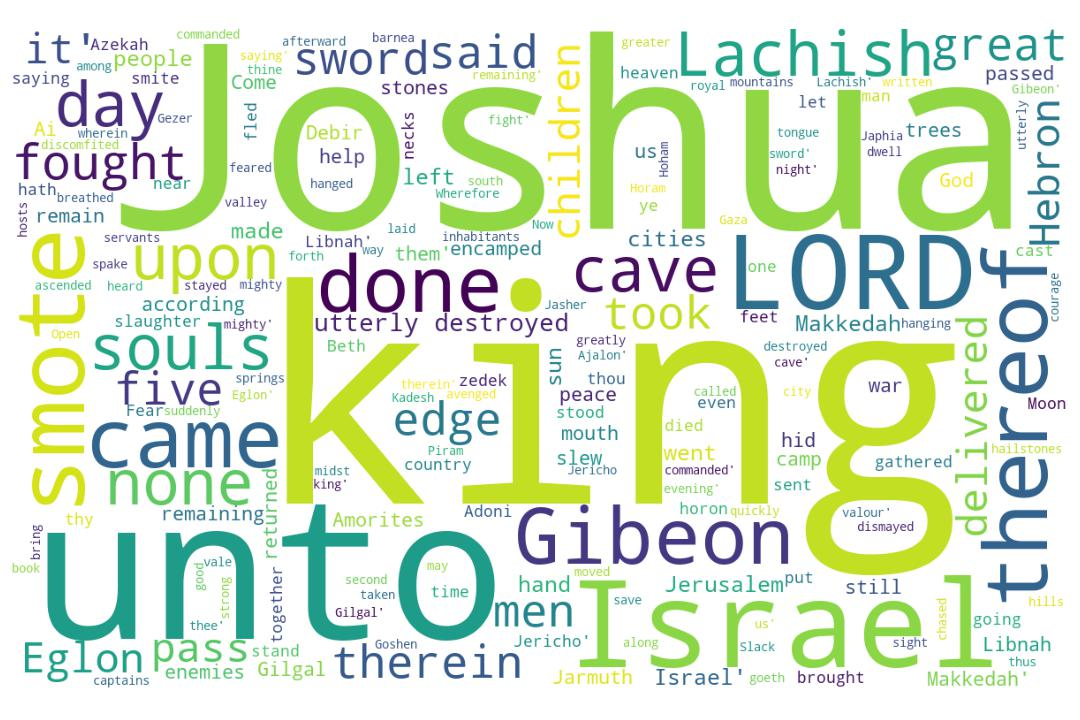
\includegraphics[width=\linewidth]{06OT-Joshua/Joshua10-WordCloud.jpg}
  \caption{Joshua 10 Word Cloud}
  \label{fig:Joshua 10 Word Cloud}
\end{figure}

\marginpar{\scriptsize \centering \fcolorbox{bone}{lime}{\textbf{THE SOUTHERN CAMPAIGN}}\\ (Joshua 10:1-43) \begin{compactenum}[I.][8]
	\item A \textbf{Strategic Advantage} \index[scripture]{Joshua!Jsh 10:01}  (Jsh 10:1) 
	\item \textbf{Solidarity} of the 5 enemy kings \index[scripture]{Joshua!Jsh 10:05}  (Jsh 10:5) 
	\item A \textbf{Surprise Attack} \index[scripture]{Joshua!Jsh 10:09}  (Jsh 10:9) 
	\item A \textbf{Slaughter} at Gibeon\index[scripture]{Joshua!Jsh 10:10}  (Jsh 10:10) 
	\item A \textbf{Stones} from heaven \index[scripture]{Joshua!Jsh 10:11}  (Jsh 10:11) 
	\item The \textbf{Stopping of the Sun} \index[scripture]{Joshua!Jsh 10:12--12}  (Jsh 10:12--13) 
	\item \textbf{Sealed} in a Cave \index[scripture]{Joshua!Jsh 10:18}  (Jsh 10:18) 
\end{compactenum}}



\footnote{\textcolor[cmyk]{0.99998,1,0,0}{\hyperlink{TOC}{Return to end of Table of Contents.}}}\footnote{\href{https://audiobible.com/bible/joshua_10.html}{\textcolor[cmyk]{0.99998,1,0,0}{Joshua 10 Audio}}}\textcolor[cmyk]{0.99998,1,0,0}{Now it came to pass, when Adoni-zedek king of Jerusalem had heard how Joshua had taken Ai, and had utterly destroyed it; as he had done to Jericho and her king, so he had done to Ai and her king; and how the inhabitants of Gibeon had made peace with Israel, and were among them;}
[2] \textcolor[cmyk]{0.99998,1,0,0}{That they feared greatly, because Gibeon \emph{was} a great city, as one of the royal cities, and because it \emph{was} greater than Ai, and all the men thereof \emph{were} mighty.}
[3] \textcolor[cmyk]{0.99998,1,0,0}{Wherefore Adoni-zedek king of Jerusalem sent unto Hoham king of Hebron, and unto Piram king of Jarmuth, and unto Japhia king of Lachish, and unto Debir king of Eglon, saying,}
[4] \textcolor[cmyk]{0.99998,1,0,0}{Come up unto me, and help me, that we may smite Gibeon: for it hath made peace with Joshua and with the children of Israel.}
[5] \textcolor[cmyk]{0.99998,1,0,0}{Therefore the five kings of the Amorites, \fcolorbox{bone}{bone}{the king of} Jerusalem, \fcolorbox{bone}{bone}{the king of} Hebron, \fcolorbox{bone}{bone}{the king of} Jarmuth, \fcolorbox{bone}{bone}{the king of} Lachish, \fcolorbox{bone}{bone}{the king of} Eglon, gathered themselves together, and went up, they and all their hosts, and encamped before Gibeon, and made war against it.}\\
\\
\P \textcolor[cmyk]{0.99998,1,0,0}{And the men of Gibeon sent unto Joshua to the camp to Gilgal, saying, Slack not thy hand from thy servants; come up to us quickly, and save us, and help us: for all the kings of the Amorites that dwell in the mountains are gathered together against us.}
[7] \textcolor[cmyk]{0.99998,1,0,0}{So Joshua ascended from Gilgal, he, and all the people of war with him, and all the mighty men of valour.}\\
\\
\P \textcolor[cmyk]{0.99998,1,0,0}{And the \fcolorbox{bone}{bone}{LORD} said unto Joshua, Fear them not: for I have delivered them into thine hand; there shall not a man of them stand before thee.}
[9] \textcolor[cmyk]{0.99998,1,0,0}{Joshua therefore came unto them suddenly, \emph{and} went up from Gilgal all night.}
[10] \textcolor[cmyk]{0.99998,1,0,0}{And the \fcolorbox{bone}{bone}{LORD} discomfited them before Israel, and slew them with a great slaughter at Gibeon, and chased them along the way that goeth up to Beth-horon, and smote them to Azekah, and unto Makkedah.}
[11] \textcolor[cmyk]{0.99998,1,0,0}{And it came to pass, as they fled from before Israel, \emph{and} were in the going down to Beth-horon, that the \fcolorbox{bone}{bone}{LORD} cast down great stones from heaven upon them unto Azekah, and they died: \emph{they} \emph{were} more which died with hailstones than \emph{they} whom the children of Israel slew with the sword.}\\
\\
\P \textcolor[cmyk]{0.99998,1,0,0}{Then spake Joshua to the \fcolorbox{bone}{bone}{LORD} in the day when the \fcolorbox{bone}{bone}{LORD} delivered up the Amorites before the children of Israel, and he said in the sight of Israel, Sun, stand thou still upon Gibeon; and thou, Moon, in the valley of Ajalon.}
[13] \textcolor[cmyk]{0.99998,1,0,0}{And the sun stood still, and the moon stayed, until the people had avenged themselves upon their enemies. \emph{Is} not this written in the book of Jasher? So the sun stood still in the midst of heaven, and hasted not to go down about a whole day.}
[14] \textcolor[cmyk]{0.99998,1,0,0}{And there was no day like that before it or after it, that the \fcolorbox{bone}{bone}{LORD} hearkened unto the voice of a man: for the \fcolorbox{bone}{bone}{LORD} fought for Israel.}\\
\\
\P \textcolor[cmyk]{0.99998,1,0,0}{And Joshua returned, and all Israel with him, unto the camp to Gilgal.}
[16] \textcolor[cmyk]{0.99998,1,0,0}{But these five kings fled, and hid themselves in a cave at Makkedah.}
[17] \textcolor[cmyk]{0.99998,1,0,0}{And it was told Joshua, saying, The five kings are found hid in a cave at Makkedah.}
[18] \textcolor[cmyk]{0.99998,1,0,0}{And Joshua said, Roll great stones upon the mouth of the cave, and set men by it for to keep them:}
[19] \textcolor[cmyk]{0.99998,1,0,0}{And stay ye not, \emph{but} pursue after your enemies, and smite the hindmost of them; suffer them not to enter into their cities: for the \fcolorbox{bone}{bone}{LORD} your God hath delivered them into your hand.}
[20] \textcolor[cmyk]{0.99998,1,0,0}{And it came to pass, when Joshua and the children of Israel had made an end of slaying them with a very great slaughter, till they were consumed, that the rest \emph{which} remained of them entered into fenced cities.}
[21] \textcolor[cmyk]{0.99998,1,0,0}{And all the people returned to the camp to Joshua at Makkedah in peace: none moved his tongue against any of the children of Israel.}
[22] \textcolor[cmyk]{0.99998,1,0,0}{Then said Joshua, Open the mouth of the cave, and bring out those five kings unto me out of the cave.}
[23] \textcolor[cmyk]{0.99998,1,0,0}{And they did so, and brought forth those five kings unto him out of the cave, \fcolorbox{bone}{bone}{the king of} Jerusalem, \fcolorbox{bone}{bone}{the king of} Hebron, \fcolorbox{bone}{bone}{the king of} Jarmuth, \fcolorbox{bone}{bone}{the king of} Lachish, \emph{and} \fcolorbox{bone}{bone}{the king of} Eglon.}
[24] \textcolor[cmyk]{0.99998,1,0,0}{And it came to pass, when they brought out those kings unto Joshua, that Joshua called for all the men of Israel, and said unto the captains of the men of war which went with him, Come near, put your feet upon the necks of these kings. And they came near, and put their feet upon the necks of them.}
[25] \textcolor[cmyk]{0.99998,1,0,0}{And Joshua said unto them, Fear not, nor be dismayed, be strong and of good courage: for thus shall the \fcolorbox{bone}{bone}{LORD} do to all your enemies against whom ye fight.}
[26] \textcolor[cmyk]{0.99998,1,0,0}{And afterward Joshua smote them, and slew them, and hanged them on five trees: and they were hanging upon the trees until the evening.}
[27] \textcolor[cmyk]{0.99998,1,0,0}{And it came to pass at the time of the going down of the sun, \emph{that} Joshua commanded, and they took them down off the trees, and cast them into the cave wherein they had been hid, and laid great stones in the cave's mouth, \emph{which} \emph{remain} until this very day.}\\
\\
\P \textcolor[cmyk]{0.99998,1,0,0}{And that day Joshua took Makkedah, and smote it with the edge of the sword, and the king thereof he utterly destroyed, them, and all the souls that \emph{were} therein; he let none remain: and he did to \fcolorbox{bone}{bone}{the king of} Makkedah as he did unto \fcolorbox{bone}{bone}{the king of} Jericho.}
[29] \textcolor[cmyk]{0.99998,1,0,0}{Then Joshua passed from Makkedah, and all Israel with him, unto Libnah, and fought against Libnah:}
[30] \textcolor[cmyk]{0.99998,1,0,0}{And the \fcolorbox{bone}{bone}{LORD} delivered it also, and the king thereof, into the hand of Israel; and he smote it with the edge of the sword, and all the souls that \emph{were} therein; he let none remain in it; but did unto the king thereof as he did unto \fcolorbox{bone}{bone}{the king of} Jericho.}\\
\\
\P \textcolor[cmyk]{0.99998,1,0,0}{And Joshua passed from Libnah, and all Israel with him, unto Lachish, and encamped against it, and fought against it:}
[32] \textcolor[cmyk]{0.99998,1,0,0}{And the \fcolorbox{bone}{bone}{LORD} delivered Lachish into the hand of Israel, which took it on the second day, and smote it with the edge of the sword, and all the souls that \emph{were} therein, according to all that he had done to Libnah.}\\
\\
\P \textcolor[cmyk]{0.99998,1,0,0}{Then Horam king of Gezer came up to help Lachish; and Joshua smote him and his people, until he had left him none remaining.}\\
\\
\P \textcolor[cmyk]{0.99998,1,0,0}{And from Lachish Joshua passed unto Eglon, and all Israel with him; and they encamped against it, and fought against it:}
[35] \textcolor[cmyk]{0.99998,1,0,0}{And they took it on that day, and smote it with the edge of the sword, and all the souls that \emph{were} therein he utterly destroyed that day, according to all that he had done to Lachish.}
[36] \textcolor[cmyk]{0.99998,1,0,0}{And Joshua went up from Eglon, and all Israel with him, unto Hebron; and they fought against it:}
[37] \textcolor[cmyk]{0.99998,1,0,0}{And they took it, and smote it with the edge of the sword, and the king thereof, and all the cities thereof, and all the souls that \emph{were} therein; he left none remaining, according to all that he had done to Eglon; but destroyed it utterly, and all the souls that \emph{were} therein.}\\
\\
\P \textcolor[cmyk]{0.99998,1,0,0}{And Joshua returned, and all Israel with him, to Debir; and fought against it:}
[39] \textcolor[cmyk]{0.99998,1,0,0}{And he took it, and the king thereof, and all the cities thereof; and they smote them with the edge of the sword, and utterly destroyed all the souls that \emph{were} therein; he left none remaining: as he had done to Hebron, so he did to Debir, and to the king thereof; as he had done also to Libnah, and to her king.}\\
\\
\P \textcolor[cmyk]{0.99998,1,0,0}{So Joshua smote all the country of the hills, and of the south, and of the vale, and of the springs, and all their kings: he left none remaining, but utterly destroyed all that breathed, as the \fcolorbox{bone}{bone}{LORD} God of Israel commanded.}
[41] \textcolor[cmyk]{0.99998,1,0,0}{And Joshua smote them from Kadesh-barnea even unto Gaza, and all the country of Goshen, even unto Gibeon.}
[42] \textcolor[cmyk]{0.99998,1,0,0}{And all these kings and their land did Joshua take at one time, because the \fcolorbox{bone}{bone}{LORD} God of Israel fought for Israel.}
[43] \textcolor[cmyk]{0.99998,1,0,0}{And Joshua returned, and all Israel with him, unto the camp to Gilgal.}

\chapter{Joshua 11}

\begin{figure}
  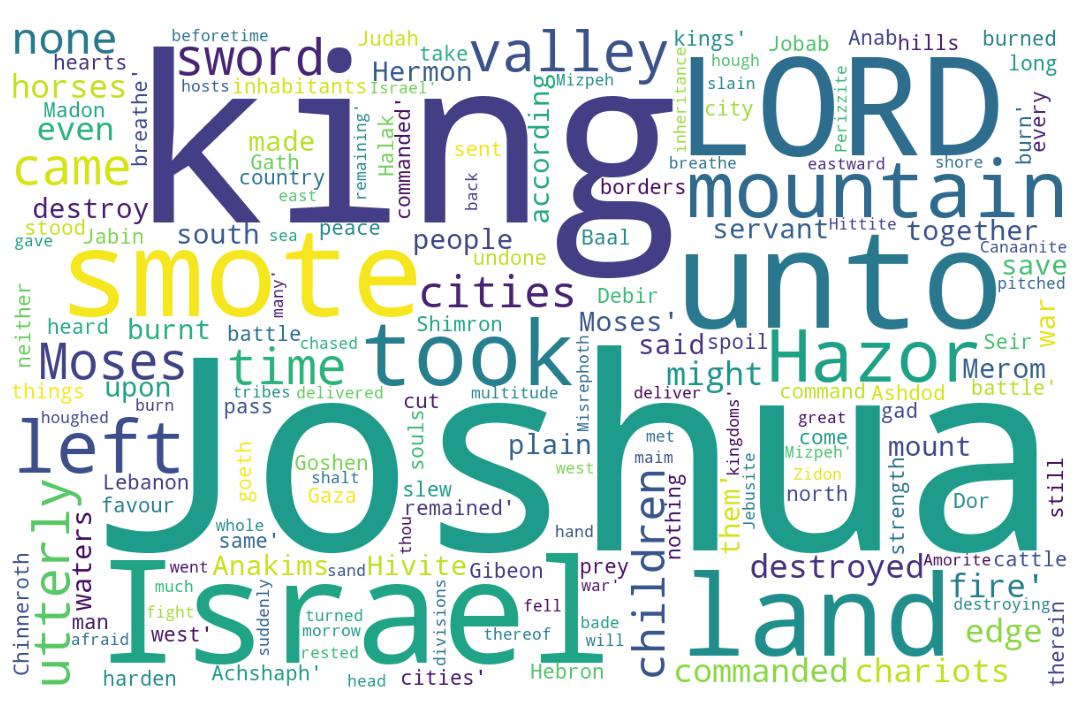
\includegraphics[width=\linewidth]{06OT-Joshua/Joshua11-WordCloud.jpg}
  \caption{Joshua 11 Word Cloud}
  \label{fig:Joshua 11 Word Cloud}
\end{figure}

\marginpar{\scriptsize \centering \fcolorbox{bone}{lime}{\textbf{THE SOUTHERN CAMPAIGN}}\\ (Joshua 11) \begin{compactenum}[I.][8]
	\item \textbf{Responisbility to Fight} \index[scripture]{Joshua!Jsh 11:01}  (Jsh 11:1) 
	\item The Enemy's \textbf{Resources} \index[scripture]{Joshua!Jsh 11:04}  (Jsh 11:4)
	\item The Enemy's \textbf{Resistance} \index[scripture]{Joshua!Jsh 11:05}  (Jsh 11:5)
	\item The \textbf{Readiness} to Fight the Long Battles \index[scripture]{Joshua!Jsh 11:18}  (Jsh 11:18)
	\item The \textbf{Reknowned} Giants \index[scripture]{Joshua!Jsh 11:21}  (Jsh 11:21)
	\item  Where the Enemy \textbf{Remained}  \index[scripture]{Joshua!Jsh 11:22}  (Jsh 11:22)
	\item  \textbf{Rest} in the Land \index[scripture]{Joshua!Jsh 11:23}  (Jsh 11:23)
\end{compactenum}}




\footnote{\textcolor[rgb]{0.00,0.25,0.00}{\hyperlink{TOC}{Return to end of Table of Contents.}}}\footnote{\href{https://audiobible.com/bible/joshua_11.html}{\textcolor[cmyk]{0.99998,1,0,0}{Joshua 11 Audio}}}\textcolor[cmyk]{0.99998,1,0,0}{\fcolorbox{bone}{bone}{And} it came \fcolorbox{bone}{bone}{to} pass, when Jabin king of Hazor had heard \emph{those} \emph{things}, that he sent \fcolorbox{bone}{bone}{to} Jobab king of Madon, and \fcolorbox{bone}{bone}{to} the king of Shimron, and \fcolorbox{bone}{bone}{to} the king of Achshaph,}
[2] \textcolor[cmyk]{0.99998,1,0,0}{\fcolorbox{bone}{bone}{And} \fcolorbox{bone}{bone}{to} the kings that \emph{were} on the north of the mountains, and of the plains south of Chinneroth, and \fcolorbox{bone}{bone}{in} the valley, and \fcolorbox{bone}{bone}{in} the borders of Dor on the west,}
[3] \textcolor[cmyk]{0.99998,1,0,0}{\emph{And} \emph{to} the Canaanite on the east and on the west, and \emph{to} the Amorite, and the Hittite, and the Perizzite, and the Jebusite \fcolorbox{bone}{bone}{in} the mountains, and \emph{to} the Hivite under Hermon \fcolorbox{bone}{bone}{in} the land of Mizpeh.}
[4] \textcolor[cmyk]{0.99998,1,0,0}{\fcolorbox{bone}{bone}{And} \fcolorbox{bone}{bone}{they} went out, \fcolorbox{bone}{bone}{they} and all their hosts \fcolorbox{bone}{bone}{with} them, much people, even as the sand that \emph{is} upon the sea shore \fcolorbox{bone}{bone}{in} multitude, \fcolorbox{bone}{bone}{with} horses and chariots very many.}
[5] \textcolor[cmyk]{0.99998,1,0,0}{\fcolorbox{bone}{bone}{And} when all these kings were met together, \fcolorbox{bone}{bone}{they} came and pitched together at the waters of Merom, \fcolorbox{bone}{bone}{to} fight against Israel.}\\
\\
\P \textcolor[cmyk]{0.99998,1,0,0}{\fcolorbox{bone}{bone}{And} the LORD said unto Joshua, Be not afraid because of them: for \fcolorbox{bone}{bone}{to} morrow about this time will I deliver them up all slain before Israel: thou shalt hough their horses, and burn their chariots \fcolorbox{bone}{bone}{with} fire.}
[7] \textcolor[cmyk]{0.99998,1,0,0}{So Joshua came, and all the people of war \fcolorbox{bone}{bone}{with} him, against them by the waters of Merom suddenly; and \fcolorbox{bone}{bone}{they} fell upon them.}
[8] \textcolor[cmyk]{0.99998,1,0,0}{\fcolorbox{bone}{bone}{And} the LORD delivered them into the hand of Israel, who smote them, and chased them unto great Zidon, and unto Misrephoth-maim, and unto the valley of Mizpeh eastward; and \fcolorbox{bone}{bone}{they} smote them, until \fcolorbox{bone}{bone}{they} left them none remaining.}
[9] \textcolor[cmyk]{0.99998,1,0,0}{\fcolorbox{bone}{bone}{And} Joshua did unto them as the LORD bade him: he houghed their horses, and burnt their chariots \fcolorbox{bone}{bone}{with} fire.}\\
\\
\P \textcolor[cmyk]{0.99998,1,0,0}{\fcolorbox{bone}{bone}{And} Joshua at that time turned back, and took Hazor, and smote the king thereof \fcolorbox{bone}{bone}{with} the sword: for Hazor beforetime was the head of all those kingdoms.}
[11] \textcolor[cmyk]{0.99998,1,0,0}{\fcolorbox{bone}{bone}{And} \fcolorbox{bone}{bone}{they} smote all the souls that \emph{were} therein \fcolorbox{bone}{bone}{with} the edge of the sword, utterly destroying \emph{them}: there was not any left \fcolorbox{bone}{bone}{to} breathe: and he burnt Hazor \fcolorbox{bone}{bone}{with} fire.}
[12] \textcolor[cmyk]{0.99998,1,0,0}{\fcolorbox{bone}{bone}{And} all the cities of those kings, and all the kings of them, did Joshua take, and smote them \fcolorbox{bone}{bone}{with} the edge of the sword, \emph{and} he utterly destroyed them, as Moses the servant of the LORD commanded.}
[13] \textcolor[cmyk]{0.99998,1,0,0}{But \emph{as} \emph{for} the cities that stood still \fcolorbox{bone}{bone}{in} their strength, Israel burned none of them, save Hazor only; \emph{that} did Joshua burn.}
[14] \textcolor[cmyk]{0.99998,1,0,0}{\fcolorbox{bone}{bone}{And} all the spoil of these cities, and the cattle, the children of Israel took for a prey unto themselves; but every man \fcolorbox{bone}{bone}{they} smote \fcolorbox{bone}{bone}{with} the edge of the sword, until \fcolorbox{bone}{bone}{they} had destroyed them, neither left \fcolorbox{bone}{bone}{they} any \fcolorbox{bone}{bone}{to} breathe.}\\
\\
\P \textcolor[cmyk]{0.99998,1,0,0}{As the LORD commanded Moses his servant, so did Moses command Joshua, and so did Joshua; he left nothing undone of all that the LORD commanded Moses.}
[16] \textcolor[cmyk]{0.99998,1,0,0}{So Joshua took all that land, the hills, and all the south country, and all the land of Goshen, and the valley, and the plain, and the mountain of Israel, and the valley of the same;}
[17] \textcolor[cmyk]{0.99998,1,0,0}{\emph{Even} from the mount Halak, that goeth up \fcolorbox{bone}{bone}{to} Seir, even unto Baal-gad \fcolorbox{bone}{bone}{in} the valley of Lebanon under mount Hermon: and all their kings he took, and smote them, and slew them.}
[18] \textcolor[cmyk]{0.99998,1,0,0}{Joshua made war a long time \fcolorbox{bone}{bone}{with} all those kings.}
[19] \textcolor[cmyk]{0.99998,1,0,0}{There was not a city that made peace \fcolorbox{bone}{bone}{with} the children of Israel, save the Hivites the inhabitants of Gibeon: all \emph{other} \fcolorbox{bone}{bone}{they} took \fcolorbox{bone}{bone}{in} battle.}
[20] \textcolor[cmyk]{0.99998,1,0,0}{For it was of the LORD \fcolorbox{bone}{bone}{to} harden their hearts, that \fcolorbox{bone}{bone}{they} should come against Israel \fcolorbox{bone}{bone}{in} battle, that he might destroy them utterly, \emph{and} that \fcolorbox{bone}{bone}{they} might have no favour, but that he might destroy them, as the LORD commanded Moses.}\\
\\
\P \textcolor[cmyk]{0.99998,1,0,0}{\fcolorbox{bone}{bone}{And} at that time came Joshua, and cut off the Anakims from the mountains, from Hebron, from Debir, from Anab, and from all the mountains of Judah, and from all the mountains of Israel: Joshua destroyed them utterly \fcolorbox{bone}{bone}{with} their cities.}
[22] \textcolor[cmyk]{0.99998,1,0,0}{There was none of the Anakims left \fcolorbox{bone}{bone}{in} the land of the children of Israel: only \fcolorbox{bone}{bone}{in} Gaza, \fcolorbox{bone}{bone}{in} Gath, and \fcolorbox{bone}{bone}{in} Ashdod, there remained.}
[23] \textcolor[cmyk]{0.99998,1,0,0}{So Joshua took the whole land, according \fcolorbox{bone}{bone}{to} all that the LORD said unto Moses; and Joshua gave it for an inheritance unto Israel according \fcolorbox{bone}{bone}{to} their divisions by their tribes. \fcolorbox{bone}{bone}{And} the land rested from war.}
\chapter{Joshua 12}

\begin{figure}
  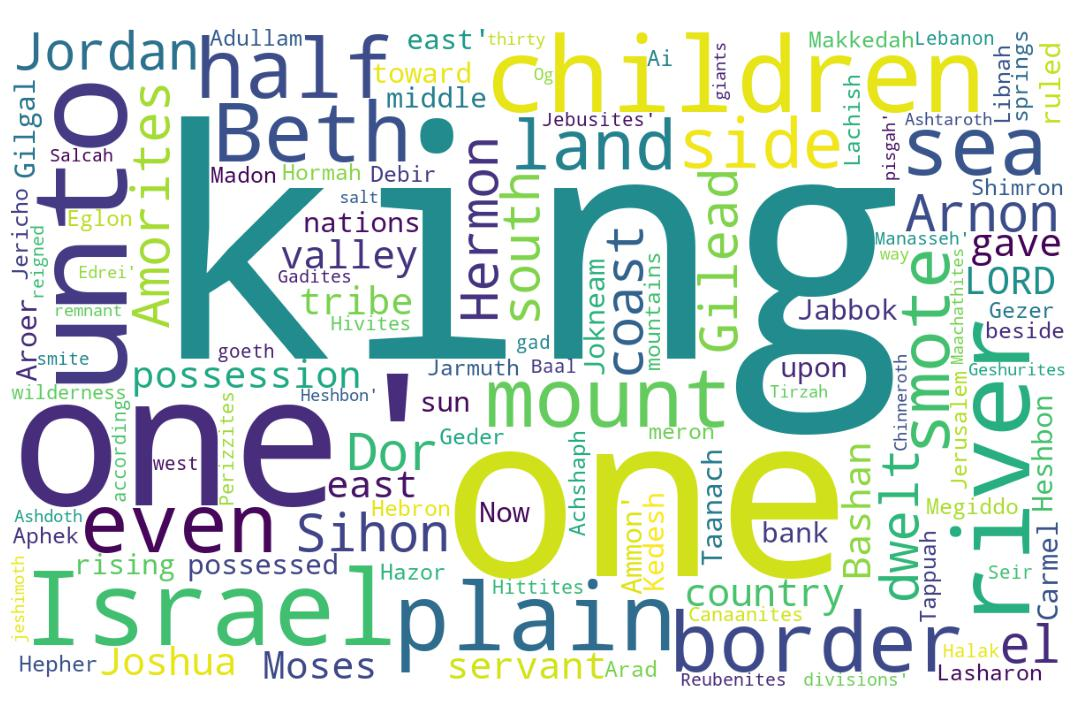
\includegraphics[width=\linewidth]{06OT-Joshua/Joshua12-WordCloud.jpg}
  \caption{Joshua 12 Word Cloud}
  \label{fig:Joshua 12 Word Cloud}
\end{figure}

\marginpar{\scriptsize \centering \fcolorbox{bone}{lime}{\textbf{A RECAP}}\\ (Joshua 12)

\begin{compactenum}[I.][8]

	\item \textbf{These} Ones Defeated  \index[scripture]{Joshua!Jsh 12:01}  (Jsh 12:1, 7) 
	\item \textbf{Tribes} On the Other Side  \index[scripture]{Joshua!Jsh 12:06}  (Jsh 12:6) 
	\item The \textbf{Terrain}  \index[scripture]{Joshua!Jsh 12:08}  (Jsh 12:8) 	
	\item \textbf{Thoughtful} Reflection -- take some time to consider the victories Gad has wrought in your life %\index[scripture]{Joshua!Jsh 12:24}  (Jsh 12:24) 
	\item \textbf{Thirty-One} Kings  \index[scripture]{Joshua!Jsh 12:10-24}  (Jsh 12:10-24) 

\end{compactenum}}





\footnote{\textcolor[cmyk]{0.99998,1,0,0}{\hyperlink{TOC}{Return to end of Table of Contents.}}}\footnote{\href{https://audiobible.com/bible/joshua_12.html}{\textcolor[cmyk]{0.99998,1,0,0}{Joshua 12 Audio}}}\textcolor[cmyk]{0.99998,1,0,0}{Now \fcolorbox{bone}{lime}{these} \emph{are} the kings of the land, which the children of Israel smote, and possessed their land on the other side Jordan toward the rising of the sun, from the river Arnon unto mount Hermon, and all the plain on the east:}
[2] \textcolor[cmyk]{0.99998,1,0,0}{Sihon king of the Amorites, who dwelt in Heshbon, \emph{and} ruled from Aroer, which \emph{is} upon the bank of the river Arnon, and from the middle of the river, and from half Gilead, even unto the river Jabbok, \emph{which} \emph{is} the border of the children of Ammon;}
[3] \textcolor[cmyk]{0.99998,1,0,0}{And from the plain to the sea of Chinneroth on the east, and unto the sea of the plain, \emph{even} the salt sea on the east, the way to Beth-jeshimoth; and from the south, under Ashdoth-pisgah:}\\
\\
\textcolor[cmyk]{0.99998,1,0,0}{And the coast of Og king of Bashan, \emph{which} \emph{was} of the remnant of the giants, that dwelt at Ashtaroth and at Edrei,}
[5] \textcolor[cmyk]{0.99998,1,0,0}{And reigned in mount Hermon, and in Salcah, and in all Bashan, unto the border of the Geshurites and the Maachathites, and half Gilead, the border of Sihon king of Heshbon.}
[6] \textcolor[cmyk]{0.99998,1,0,0}{Them did Moses the servant of the LORD and the children of Israel smite: and Moses the servant of the LORD gave it \emph{for} a possession unto the Reubenites, and the Gadites, and the half \fcolorbox{bone}{lime}{tribe} of Manasseh.}
[7] \textcolor[cmyk]{0.99998,1,0,0}{And \fcolorbox{bone}{lime}{these} \emph{are} the kings of the country which Joshua and the children of Israel smote on this side Jordan on the west, from Baal-gad in the valley of Lebanon even unto the mount Halak, that goeth up to Seir; which Joshua gave unto the tribes of Israel \emph{for} a possession according to their divisions;}
[8] \textcolor[cmyk]{0.99998,1,0,0}{In the \fcolorbox{bone}{lime}{mountains}, and in the \fcolorbox{bone}{lime}{valleys}, and in the \fcolorbox{bone}{lime}{plains}, and in the \fcolorbox{bone}{lime}{springs}, and in the \fcolorbox{bone}{lime}{wilderness}, and in the \fcolorbox{bone}{lime}{south country}; the Hittites, the Amorites, and the Canaanites, the Perizzites, the Hivites, and the Jebusites:}\\
\\
\textcolor[cmyk]{0.99998,1,0,0}{The king of Jericho, one; the king of Ai, which \emph{is} beside Beth-el, one;}
[10] \textcolor[cmyk]{0.99998,1,0,0}{The king of Jerusalem, one; the king of Hebron, one;}
[11] \textcolor[cmyk]{0.99998,1,0,0}{The king of Jarmuth, one; the king of Lachish, one;}
[12] \textcolor[cmyk]{0.99998,1,0,0}{The king of Eglon, one; the king of Gezer, one;}
[13] \textcolor[cmyk]{0.99998,1,0,0}{The king of Debir, one; the king of Geder, one;}
[14] \textcolor[cmyk]{0.99998,1,0,0}{The king of Hormah, one; the king of Arad, one;}
[15] \textcolor[cmyk]{0.99998,1,0,0}{The king of Libnah, one; the king of Adullam, one;}
[16] \textcolor[cmyk]{0.99998,1,0,0}{The king of Makkedah, one; the king of Beth-el, one;}
[17] \textcolor[cmyk]{0.99998,1,0,0}{The king of Tappuah, one; the king of Hepher, one;}
[18] \textcolor[cmyk]{0.99998,1,0,0}{The king of Aphek, one; the king of Lasharon, one;}
[19] \textcolor[cmyk]{0.99998,1,0,0}{The king of Madon, one; the king of Hazor, one;}
[20] \textcolor[cmyk]{0.99998,1,0,0}{The king of Shimron-meron, one; the king of Achshaph, one;}
[21] \textcolor[cmyk]{0.99998,1,0,0}{The king of Taanach, one; the king of Megiddo, one;}
[22] \textcolor[cmyk]{0.99998,1,0,0}{The king of Kedesh, one; the king of Jokneam of Carmel, one;}
[23] \textcolor[cmyk]{0.99998,1,0,0}{The king of Dor in the coast of Dor, one; the king of the nations of Gilgal, one;}
[24] \textcolor[cmyk]{0.99998,1,0,0}{The king of Tirzah, one: all the kings thirty and one.}

\chapter{Psalm 68}

\begin{figure}
  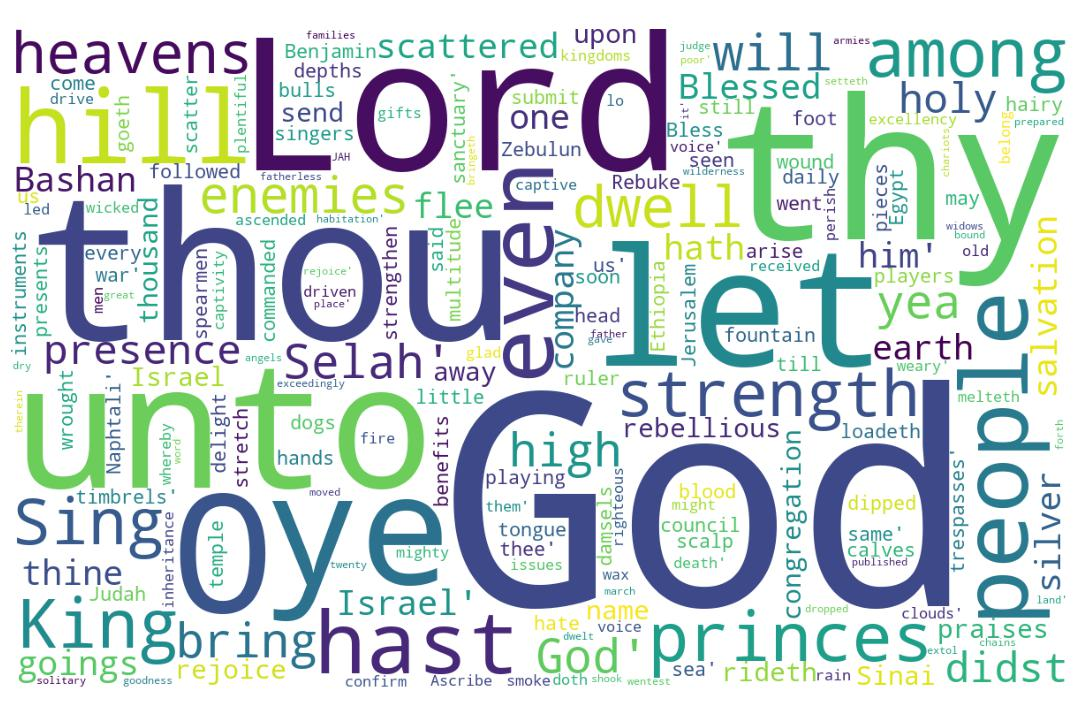
\includegraphics[width=\linewidth]{19OT-Psalms/Psalm68-WordCloud.jpg}
  \caption{Psalm 68 Word Cloud}
  \label{fig:Psalm 68 word Cloud}
\end{figure}

\marginpar{\scriptsize \centering \fcolorbox{bone}{lime}{\textbf{THINGS THAT BELONG TO GOD}}\\ (Psalm 68:1-35) \begin{compactenum}[I.][8]
    \item The \textbf{Removal} of his Enemies \index[scripture]{Psalms!Psa 068:02}(Psa 68:2)
    \item \textbf{Ministry}  \index[scripture]{Psalms!Psa 068:11}(Psa 68:11)
    \begin{compactenum}[A.]
    	\item To Captives \index[scripture]{Psalms!Psa 068:05}(Psa 68:5)
    	\item To Orphans \index[scripture]{Psalms!Psa 068:05}(Psa 68:5)
    	\item To Widows \index[scripture]{Psalms!Psa 068:05}(Psa 68:5)
    	\item To Sinners \index[scripture]{Psalms!Psa 068:20}(Psa 68:20)
    \end{compactenum}
    \item A \textbf{Message}  \index[scripture]{Psalms!Psa 068:11}(Psa 68:11)
    \item \textbf{Men}  \index[scripture]{Psalms!Psa 068:18}(Psa 68:18)
    \item Special \textbf{Music}  \index[scripture]{Psalms!Psa 068:25}(Psa 68:25)
    \item A \textbf{Millennial Reign}  \index[scripture]{Psalms!Psa 068:29}(Psa 68:29)
    \item A \textbf{Might Voice}  \index[scripture]{Psalms!Psa 068:33}(Psa 68:33)
\end{compactenum}}

\footnote{\textcolor[rgb]{0.00,0.25,0.00}{\hyperlink{TOC}{Return to end of Table of Contents.}}}\footnote{\href{https://audiobible.com/bible/psalms_68.html}{\textcolor[cmyk]{0.99998,1,0,0}{Psalm 68 Audio}}}\textcolor[cmyk]{0.99998,1,0,0}{To the chief Musician, A Psalm \emph{or} Song of David.}\\
\\
\textcolor[cmyk]{0.99998,1,0,0}{Let God arise, let his enemies be scattered: let them also that hate him flee before him.}
[2] \textcolor[cmyk]{0.99998,1,0,0}{As smoke is driven away, \emph{so} drive \emph{them} away: as wax melteth before the fire, \emph{so} let the wicked  \fcolorbox{bone}{lime}{perish} at the presence of God.}\footnote{\textbf{Psalm 97:5} - The hills melted like wax at the presence of the LORD, at the presence of the Lord of the whole earth.}\footnote{\textbf{Micah 1:4} - And the mountains shall be molten under him, and the valleys shall be cleft, as wax before the fire, and as the waters that are poured down a steep place.}
[3] \textcolor[cmyk]{0.99998,1,0,0}{But let the righteous be glad; let them rejoice before God: yea, let them exceedingly rejoice.}
[4] \textcolor[cmyk]{0.99998,1,0,0}{Sing unto God, sing praises to his name: extol him that rideth upon the heavens by his name JAH, and rejoice before him.}
[5] \textcolor[cmyk]{0.99998,1,0,0}{A father of the  \fcolorbox{bone}{lime}{fatherless}, and a judge of the  \fcolorbox{bone}{lime}{widows}, \emph{is} God in his holy habitation.}
[6] \textcolor[cmyk]{0.99998,1,0,0}{God setteth the solitary in families: he bringeth out those which are bound with chains: but the rebellious dwell in a dry \emph{land}.}
[7] \textcolor[cmyk]{0.99998,1,0,0}{O God, when thou wentest forth before thy people, when thou didst march through the wilderness; Selah:}
[8] \textcolor[cmyk]{0.99998,1,0,0}{The earth shook, the heavens also dropped at the presence of God: \emph{even} Sinai itself \emph{was} \emph{moved} at the presence of God, the God of Israel.}
[9] \textcolor[cmyk]{0.99998,1,0,0}{Thou, O God, didst send a plentiful rain, whereby thou didst confirm thine inheritance, when it was weary.}
[10] \textcolor[cmyk]{0.99998,1,0,0}{Thy congregation hath dwelt therein: thou, O God, hast prepared of thy goodness for the poor.}
[11] \textcolor[cmyk]{0.99998,1,0,0}{The  \fcolorbox{bone}{lime}{Lord gave the word}: great \emph{was} the company of those that published \emph{it}.}
[12] \textcolor[cmyk]{0.99998,1,0,0}{Kings of armies did flee apace: and she that tarried at home divided the spoil.}
[13] \textcolor[cmyk]{0.99998,1,0,0}{Though ye have lien among the pots, \emph{yet} \emph{shall} \emph{ye} \emph{be} \emph{as} the wings of a dove covered with silver, and her feathers with lime gold.}
[14] \textcolor[cmyk]{0.99998,1,0,0}{When the Almighty scattered kings in it, it was \emph{white} as snow in Salmon.}
[15] \textcolor[cmyk]{0.99998,1,0,0}{The hill of God \emph{is} \emph{as} the hill of Bashan; an high hill \emph{as} the hill of Bashan.}
[16] \textcolor[cmyk]{0.99998,1,0,0}{Why leap ye, ye high hills? \emph{this} \emph{is} the hill \emph{which} God desireth to dwell in; yea, the LORD will dwell \emph{in} \emph{it} for ever.}
[17] \textcolor[cmyk]{0.99998,1,0,0}{The chariots of God \emph{are} twenty thousand, \emph{even} thousands of angels: the Lord \emph{is} among them, \emph{as} \emph{in} Sinai, in the holy \emph{place}.}
[18] \textcolor[cmyk]{0.99998,1,0,0}{Thou hast ascended on high, thou hast led captivity captive: thou hast received  \fcolorbox{bone}{lime}{gifts for men}; yea, \emph{for} the rebellious also, that the LORD God might dwell \emph{among} \emph{them}.}
[19] \textcolor[cmyk]{0.99998,1,0,0}{Blessed \emph{be} the Lord, \emph{who} daily loadeth us \emph{with} \emph{benefits,} \emph{even} the God of our salvation. Selah.}
[20] \textcolor[cmyk]{0.99998,1,0,0}{\emph{He} \emph{that} \emph{is} our God \emph{is} the God of  \fcolorbox{bone}{lime}{salvation}; and unto GOD the Lord \emph{belong} the issues from death.}
[21] \textcolor[cmyk]{0.99998,1,0,0}{But God shall wound the head of his enemies, \emph{and} the hairy scalp of such an one as goeth on still in his trespasses.}
[22] \textcolor[cmyk]{0.99998,1,0,0}{The Lord said, I will bring again from Bashan, I will bring \emph{my} \emph{people} again from the depths of the sea:}
[23] \textcolor[cmyk]{0.99998,1,0,0}{That thy foot may be dipped in the blood of \emph{thine} enemies, \emph{and} the tongue of thy dogs in the same.}
[24] \textcolor[cmyk]{0.99998,1,0,0}{They have seen thy goings, O God; \emph{even} the goings of my God, my King, in the sanctuary.}
[25] \textcolor[cmyk]{0.99998,1,0,0}{The  \fcolorbox{bone}{lime}{singers} went before, the players on  \fcolorbox{bone}{lime}{instruments} \emph{followed} after; among \emph{them} \emph{were} the damsels playing with  \fcolorbox{bone}{lime}{timbrels}.}
[26] \textcolor[cmyk]{0.99998,1,0,0}{Bless ye God in the \fcolorbox{bone}{MYGOLD}{congregations}, \emph{even} the Lord, from the fountain of Israel.}
[27] \textcolor[cmyk]{0.99998,1,0,0}{There \emph{is} little Benjamin \emph{with} their ruler, the princes of Judah \emph{and} their council, the princes of Zebulun, \emph{and} the princes of Naphtali.}
[28] \textcolor[cmyk]{0.99998,1,0,0}{Thy God hath commanded thy strength: strengthen, O God, that which thou hast wrought for us.}
[29] \textcolor[cmyk]{0.99998,1,0,0}{Because of thy  \fcolorbox{bone}{lime}{temple} at Jerusalem shall kings bring presents unto thee.}
[30] \textcolor[cmyk]{0.99998,1,0,0}{Rebuke the company of spearmen, the multitude of the bulls, with the calves of the people, \emph{till} \emph{every} \emph{one} submit himself with pieces of silver: scatter thou the people \emph{that} delight in war.}
[31] \textcolor[cmyk]{0.99998,1,0,0}{Princes shall come out of Egypt; Ethiopia shall soon stretch out her hands unto God.}
[32] \textcolor[cmyk]{0.99998,1,0,0}{Sing unto God, ye kingdoms of the earth; O sing praises unto the Lord; Selah:}
[33] \textcolor[cmyk]{0.99998,1,0,0}{To him that rideth upon the heavens of heavens, \emph{which} \emph{were} of old; lo, he doth send out his  \fcolorbox{bone}{lime}{voice}, \emph{and} \emph{that} a mighty  \fcolorbox{bone}{lime}{voice}.}
[34] \textcolor[cmyk]{0.99998,1,0,0}{Ascribe ye strength unto God: his excellency \emph{is} over Israel, and his strength \emph{is} in the clouds.}
[35] \textcolor[cmyk]{0.99998,1,0,0}{O God, \emph{thou} \emph{art} terrible out of thy holy places: the God of Israel \emph{is} he that giveth strength and power unto \emph{his} people. Blessed \emph{be} God.}

\chapter{Proverb 9}

\begin{figure}
  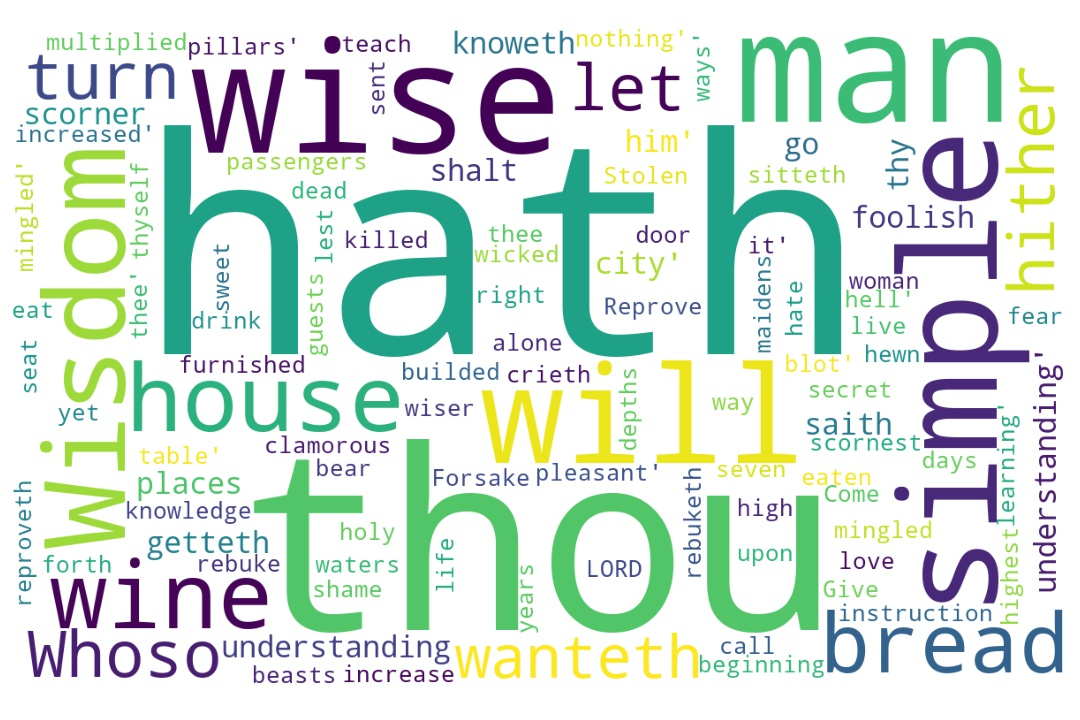
\includegraphics[width=\linewidth]{20OT-Proverbs/Proverb9-WordCloud.jpg}
  \caption{Proverb 9 Word Cloud}
  \label{fig:Proverb 9 Word Cloud}
\end{figure}


\marginpar{\scriptsize \centering \fcolorbox{bone}{lime}{\textbf{WISDOM: THE GOOD CHOICE}}\\ (Proverb 9:1-18) \begin{compactenum}[I.][8]
\item \textbf{Builds} a Life \index[scripture]{Proverbs!Pro 09:01}(Pro 9:1)
\item Has a \textbf{Banquet} \index[scripture]{Proverbs!Pro 09:02}(Pro 9:2)
\item Gives out \textbf{Bread} \index[scripture]{Proverbs!Pro 09:05}(Pro 9:5)
\item Has \textbf{Blessings} \index[scripture]{Proverbs!Pro 09:09}(Pro 9:9)
\item Was there from the \textbf{Beginning} \index[scripture]{Proverbs!Pro 09:10}(Pro 9:10)
\item Provides Lasting \textbf{Benefits} \index[scripture]{Proverbs!Pro 09:11}(Pro 9:11)
\item Is \textbf{Betrayed} \index[scripture]{Proverbs!Pro 09:13}(Pro 9:13)
\end{compactenum}}

\marginpar{\scriptsize \centering \fcolorbox{bone}{yellow}{\textbf{WISDOM AT WORK}}\\ (Proverb 9:1-18) \begin{compactenum}[I.][8]
    \item \textbf{Builds a House} \index[scripture]{Proverbs!Pro 09:01}(Pro 9:1)
    \item \textbf{Hews out Pillars} \index[scripture]{Proverbs!Pro 09:01}(Pro 9:1)
    \item \textbf{Kills her Beats} \index[scripture]{Proverbs!Pro 09:02}(Pro 9:2)
    \item \textbf{Mingles Her Wine} \index[scripture]{Proverbs!Pro 09:02}(Pro 9:2)
    \item \textbf{Furnishes her Table} \index[scripture]{Proverbs!Pro 09:02}(Pro 9:2)
    \item \textbf{Sends forthe her Maidens} \index[scripture]{Proverbs!Pro 09:03}(Pro 9:3)
    \item \textbf{Cries from the High Places} \index[scripture]{Proverbs!Pro 09:03}(Pro 9:3)
\end{compactenum}}

\marginpar{\scriptsize \centering \fcolorbox{bone}{black}{\textbf{\textcolor[cmyk]{0,0,0,0}{LOOKING FOR WISDOM}}}\\ (Proverb 9) 
\begin{compactenum}[I.][8]
    \item The \textbf{Rendering of Wisdom} \index[scripture]{Proverbs!Pro 09:01}(Pro 9:1) 
   \item The \textbf{Reaction to Wisdom} \index[scripture]{Proverbs!Pro 09:09}(Pro 9:9) 
    \item The \textbf{Reach for Wisdom} \index[scripture]{Proverbs!Pro 09:10}(Pro 9:10) 
    \item The \textbf{Road to Wisdom} \index[scripture]{Proverbs!Pro 09:11}(Pro 9:11) 
    \item The \textbf{Rejection of Wisdom} \index[scripture]{Proverbs!Pro 09:13}(Pro 9:13) 
    \item Man's \textbf{Regard \& Reverence for Foolishness} \index[scripture]{Proverbs!Pro 09:14}(Pro 9:14) 
    \item A \textbf{Reunion of Fools} \index[scripture]{Proverbs!Pro 09:15}(Pro 9:15) 
\end{compactenum}}

\footnote{\textcolor[cmyk]{0.99998,1,0,0}{\hyperlink{TOC}{Return to end of Table of Contents.}}}\footnote{\href{https://audiobible.com/bible/proverbs_9.html}{\textcolor[cmyk]{0.99998,1,0,0}{Proverbs Audio}}}\textcolor[cmyk]{0.99998,1,0,0}{Wisdom hath \fcolorbox{bone}{lime}{builded her house}, she hath hewn out her seven pillars:}\footnote{\textbf{1 Kings 8:27} - But will God indeed dwell on the earth? behold, the heaven and heaven of heavens cannot contain thee; how much less this house that I have builded?} 
[2] \textcolor[cmyk]{0.99998,1,0,0}{She hath killed her beasts; she hath mingled her wine; she hath also \fcolorbox{bone}{lime}{furnished} her table.}
[3] \textcolor[cmyk]{0.99998,1,0,0}{She hath sent forth her maidens: she crieth upon the highest places of the city,}
[4] \textcolor[cmyk]{0.99998,1,0,0}{Whoso \emph{is} simple, let him turn in hither: \emph{as} \emph{for} him that wanteth \fcolorbox{bone}{MYGOLD}{understanding}, she saith to him,}
[5] \textcolor[cmyk]{0.99998,1,0,0}{Come, \fcolorbox{bone}{lime}{eat of my} \fcolorbox{bone}{lime}{bread}, and drink of the wine \emph{which} I have mingled.}
[6] \textcolor[cmyk]{0.99998,1,0,0}{Forsake the foolish, and live; and go in the way of \fcolorbox{bone}{MYGOLD}{understanding}.}
[7] \textcolor[cmyk]{0.99998,1,0,0}{He that reproveth a scorner getteth to himself shame: and he that rebuketh a wicked \emph{man} \emph{getteth} himself a blot.}
[8] \textcolor[cmyk]{0.99998,1,0,0}{Reprove not a scorner, lest he hate thee: rebuke a wise man, and he will love thee.}
[9] \textcolor[cmyk]{0.99998,1,0,0}{Give \emph{instruction} to a wise \emph{man}, and he will \fcolorbox{bone}{lime}{be yet wiser}: teach a just \emph{man}, and he will increase in learning.}
[10] \textcolor[cmyk]{0.99998,1,0,0}{The fear of the LORD \emph{is} the \fcolorbox{bone}{lime}{beginning of wisdom}: and the knowledge of the holy \emph{is} \fcolorbox{bone}{MYGOLD}{understanding}.}
[11] \textcolor[cmyk]{0.99998,1,0,0}{For by me thy days shall be multiplied, and the years of thy life shall be \fcolorbox{bone}{lime}{increased}.}
[12] \textcolor[cmyk]{0.99998,1,0,0}{If thou be wise, thou shalt be wise for thyself: but \emph{if} thou scornest, thou alone shalt bear \emph{it}.}
[13] \textcolor[cmyk]{0.99998,1,0,0}{A foolish woman \emph{is} clamorous: \emph{she} \emph{is} simple, and \fcolorbox{bone}{lime}{knoweth nothing}.}
[14] \textcolor[cmyk]{0.99998,1,0,0}{For she sitteth at the door of her house, on a seat in the high places of the city,}
[15] \textcolor[cmyk]{0.99998,1,0,0}{To call passengers who go right on their ways:}
[16] \textcolor[cmyk]{0.99998,1,0,0}{Whoso \emph{is} simple, let him turn in hither: and \emph{as} \emph{for} him that wanteth \fcolorbox{bone}{MYGOLD}{understanding}, she saith to him,}
[17] \textcolor[cmyk]{0.99998,1,0,0}{Stolen waters are sweet, and bread \emph{eaten} in secret is pleasant.}
[18] \textcolor[cmyk]{0.99998,1,0,0}{But he knoweth not that the dead \emph{are} there; \emph{and} \emph{that} her guests \emph{are} in the depths of hell.}




\end{document}

